%%%%%%%%%%%%%%%%%%%%%%%%%%%%%%%%%%%%%%%%%
% University/School Laboratory Report
% LaTeX Template
% Version 3.1 (25/3/14)
%
% This template has been downloaded from:
% http://www.LaTeXTemplates.com
%
% Original author:
% Linux and Unix Users Group at Virginia Tech Wiki 
% (https://vtluug.org/wiki/Example_LaTeX_chem_lab_report)
%
% License:
% CC BY-NC-SA 3.0 (http://creativecommons.org/licenses/by-nc-sa/3.0/)
%
%%%%%%%%%%%%%%%%%%%%%%%%%%%%%%%%%%%%%%%%%

%----------------------------------------------------------------------------------------
%	PACKAGES AND DOCUMENT CONFIGURATIONS
%----------------------------------------------------------------------------------------

\documentclass[12pt]{article}
\usepackage[left=3cm, right=3cm]{geometry}

\usepackage[version=3]{mhchem} % Package for chemical equation typesetting
\usepackage{siunitx} % Provides the \SI{}{} and \si{} command for typesetting SI units
\usepackage{natbib} % Required to change bibliography style to APA
\usepackage{amsmath} % Required for some math elements 
\usepackage{tabularx,booktabs,tabulary,array,graphicx,url}
\usepackage{graphicx}
\usepackage{multirow}
%\usepackage{caption}
%\usepackage{subcaption}
\usepackage{subfig}
\newcommand*\rot{\rotatebox{90}}

\setlength\parindent{0pt} % Removes all indentation from paragraphs

\renewcommand{\labelenumi}{\alph{enumi}.} % Make numbering in the enumerate environment by letter rather than number (e.g. section 6)

%\usepackage{times} % Uncomment to use the Times New Roman font

%----------------------------------------------------------------------------------------
%	DOCUMENT INFORMATION
%----------------------------------------------------------------------------------------

\title{Correction of keyboard typos with an Hidden Markov Model} % Title

\author{Ilaria Pigazzini, Cezar Angelo Sas, Andrea Vidali} %
% Author name

\date{\today} % Date for the report

\begin{document}

\maketitle % Insert the title, author and date

% \begin{center}
% \begin{tabular}{l r}
% Date Performed: & January 1, 2012 \\ % Date the experiment was performed
% Partners: & James Smith \\ % Partner names
% & Mary Smith \\
% Instructor: & Professor Smith % Instructor/supervisor
% \end{tabular}
% \end{center}

% If you wish to include an abstract, uncomment the lines below
% \begin{abstract}
% Abstract text
% \end{abstract}

%----------------------------------------------------------------------------------------
%	SECTION 1
%----------------------------------------------------------------------------------------
\newpage
\tableofcontents \newpage
\section{Introduction}
HMMispelling is a demo application to correct input keyboard typos. During the
development of our project we made some studies on the problem: we defined an
Hidden Markov Model, ran the Viterbi algorithm on it and analyzed the
results by comparing different configurations and inputs.
% To determine the atomic weight of magnesium via its reaction with oxygen and to study the stoichiometry of the reaction (as defined in \ref{definitions}):
% 
% \begin{center}\ce{2 Mg + O2 -> 2 MgO}\end{center}

% If you have more than one objective, uncomment the below:
%\begin{description}
%\item[First Objective] \hfill \\
%Objective 1 text
%\item[Second Objective] \hfill \\
%Objective 2 text
%\end{description}

\section{The model}
We modeled the problem as an hidden markov model, where the hidden states are
the characters of the text which should have been typed; the emissions are the
actual typed characters.
\subsection{Inference task: Viterbi}
The chosen task to infer the correct typed text is �Most Likely Sequence�. The
Hidden Markov Model library(see Section~\ref{libraries}, Hidden-Markov Model) used in our
project implements the Viterbi algorithm.
% \label{definitions}
% \begin{description}
% \item[Stoichiometry]
% The relationship between the relative quantities of substances taking part in a reaction or forming a compound, typically a ratio of whole integers.
% \item[Atomic mass]
% The mass of an atom of a chemical element expressed in atomic mass units. It is approximately equivalent to the number of protons and neutrons in the atom (the mass number) or to the average number allowing for the relative abundances of different isotopes. 
% \end{description} 
 
%----------------------------------------------------------------------------------------
%	SECTION 2
%----------------------------------------------------------------------------------------
\subsection{Model Parameters}
% Table generated by Excel2LaTeX from sheet 'Foglio4'
Following, the parameters given to the model:
\begin{itemize}
	\item[]\emph{States}: alphabetical characters of the $QWERTY$ keyboard
	\item[]\emph{Emissions}: alphabetical characters of the $QWERTY$ keyboard
	\item[]\emph{Prior Probability Matrix}: relative frequencies of letters in the
	Englis language.
	\item[]\emph{Transition Matrix}: bigram frequencies of the English language. 
	See Section~\ref{transitionM} for further information.
	\item[]\emph{Emission Matrix}: the probability of the digit to be correct or
	uncorrect. The uncorrect digits for every QWERTY alphabetical character are its
	neighbors with distance one. See Section~\ref{emissionM} for further
	information.
\end{itemize}
Since the correction of mispelling will be applied on the alphabetical
characters(lowercase and uppercase, plus whitespace) of the $QWERTY$ keyboard,
in the following sections we will refer to keyboard input as ``digit''.
\subsection{Transition matrix}\label{transitionM}
%how we obtained it
The transition matrix describes the probability of a digit to be followed by
another digit in the input text. The values of this matrix are bigram
frequencies of the English language, where a bigram is a sequence of two digits.
We trained this matrix on three datasets: \emph{Swift}, \emph{Twitter} and the
sum of the two, named \emph{Hybrid}(see Section~\ref{dataset}).
\subsection{Emission matrix}\label{emissionM}
%list the 3 different types
Consider a digit of the keyboard. In our model we assume that its neighbors are
all digit placed at distance ``$1$ digit'' in every direction on the keyboard.
For instance, digit ``$S$'' is at distance $1$ from digit ``$A$'' but it is at distance ``$2$'' from
digit ``$F$''.

Given the intention of press a digit on the keyboard and all the digits, the
emission matrix describes the probability of a digit to be press given the will
of press the intended digit~(``fat finger typo''). For each digit, this matrix
contains relevant values when the probability refers to the neighbor digits of
the intended digit. The other probabilities are set to constant $\epsilon =
10^{-5}$.

We modeled the neighbors of every digit as a $3$x$3$ neighbor matrix
where the intended digit is placed in position $[2, 2]$ (See
Figure~\ref{neighborM}). If a digit is on the edge of the keyboard, the position
contains a $null$ value. Given a neighbor matrix, we compute a bidimensional
distribution centered on the intended digit position.
We tested three different kinds of distribution: uniform, gaussian and custom.
For what concerns the uniform distribution, we assumed that every neighbor digit
and the intended one have the same probability to be press. This
simplified configuration led to poor results, since there is no emphasis on the
fact that the intended digit will be press correctly most of the time.
This problem was solved by introducing the gaussian distribution with $mean$
equals to $0$(Figure~\ref{gaussianD}. We explored different settings for the
$variance$ in order to find the best configuration~(see Section \ref{analysis}). Even if the gaussian
distribution seems to offer good values for the emission matrix, it should
be used to model continous variables.

Finally, we tested our custom distribution where the probability of press the
intended digit is definitely higher than the probability of press its neighbors,
which is uniform. This distribution gave the best results.

% \begin{figure}%[hbp]
% \centering
% \begin{minipage}{.5\textwidth}
% \centering
% 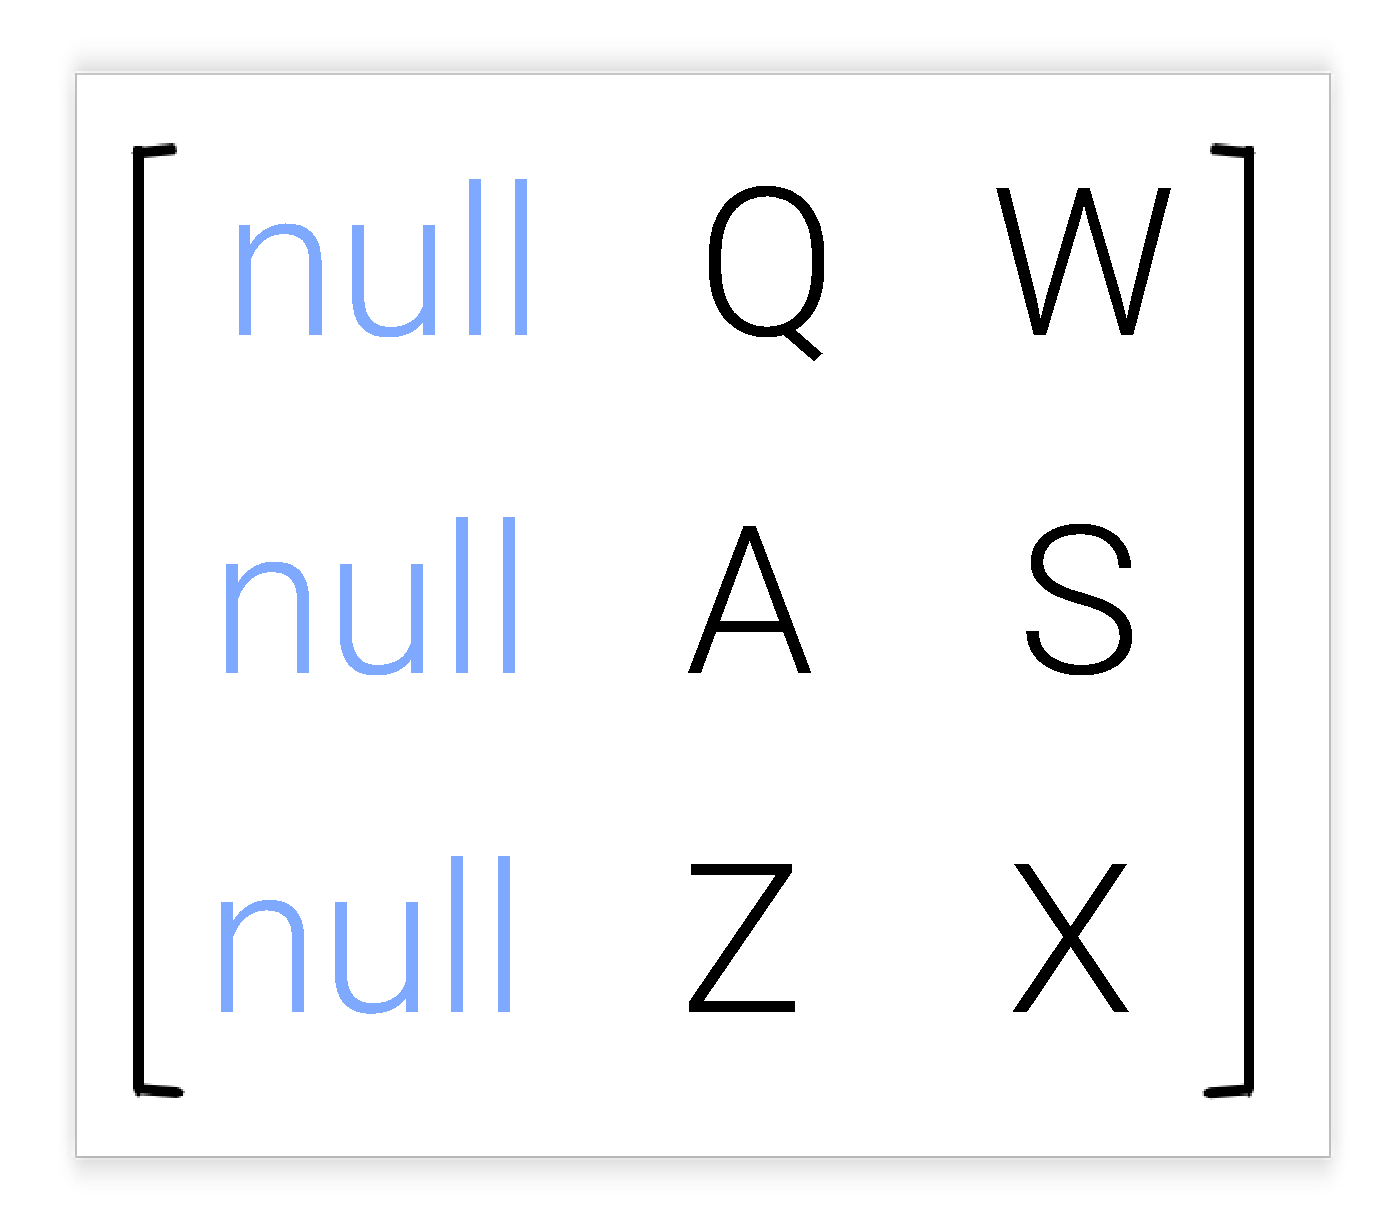
\includegraphics[width=0.5\linewidth,clip=true,trim=0 0 0
% 0]{neighbor_matrix.pdf}
% \caption{Neighbor matrix}
% \label{neighborM}
% \end{minipage}
% \hfill
% \begin{minipage}{.5\textwidth}
% \centering
% 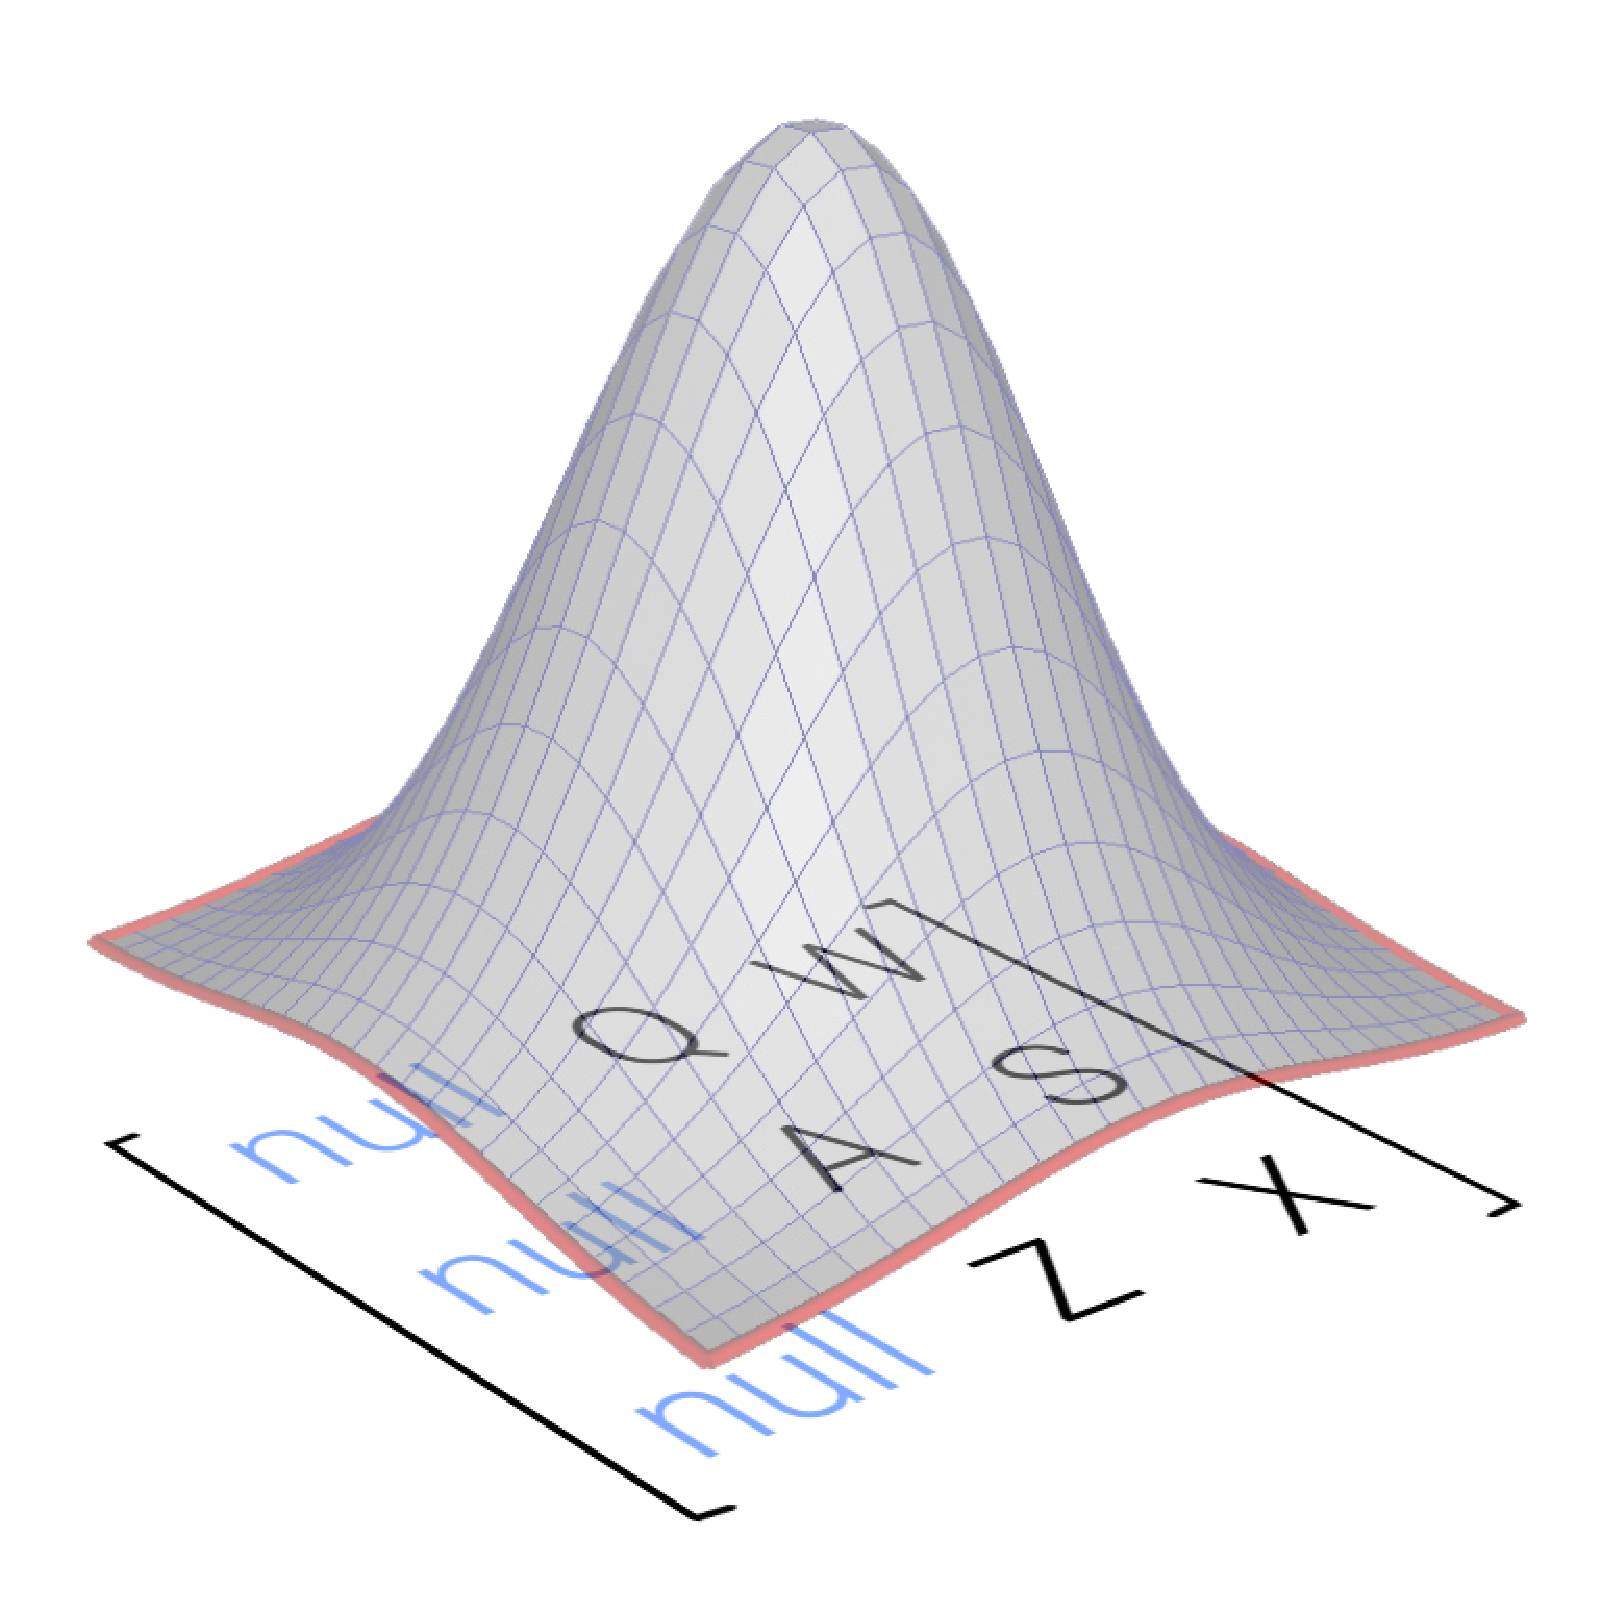
\includegraphics[width=0.5\linewidth,clip=true,trim=0 0 0
% 0]{3D_Gaussian_Perspective.pdf}
% \caption{Gaussian distribution example}
% \label{gaussianD}
% \end{minipage}
% \end{figure}

\begin{figure}[!htbp]
\centering
\subfloat[][Neighbor matrix \label{neighborM}]
{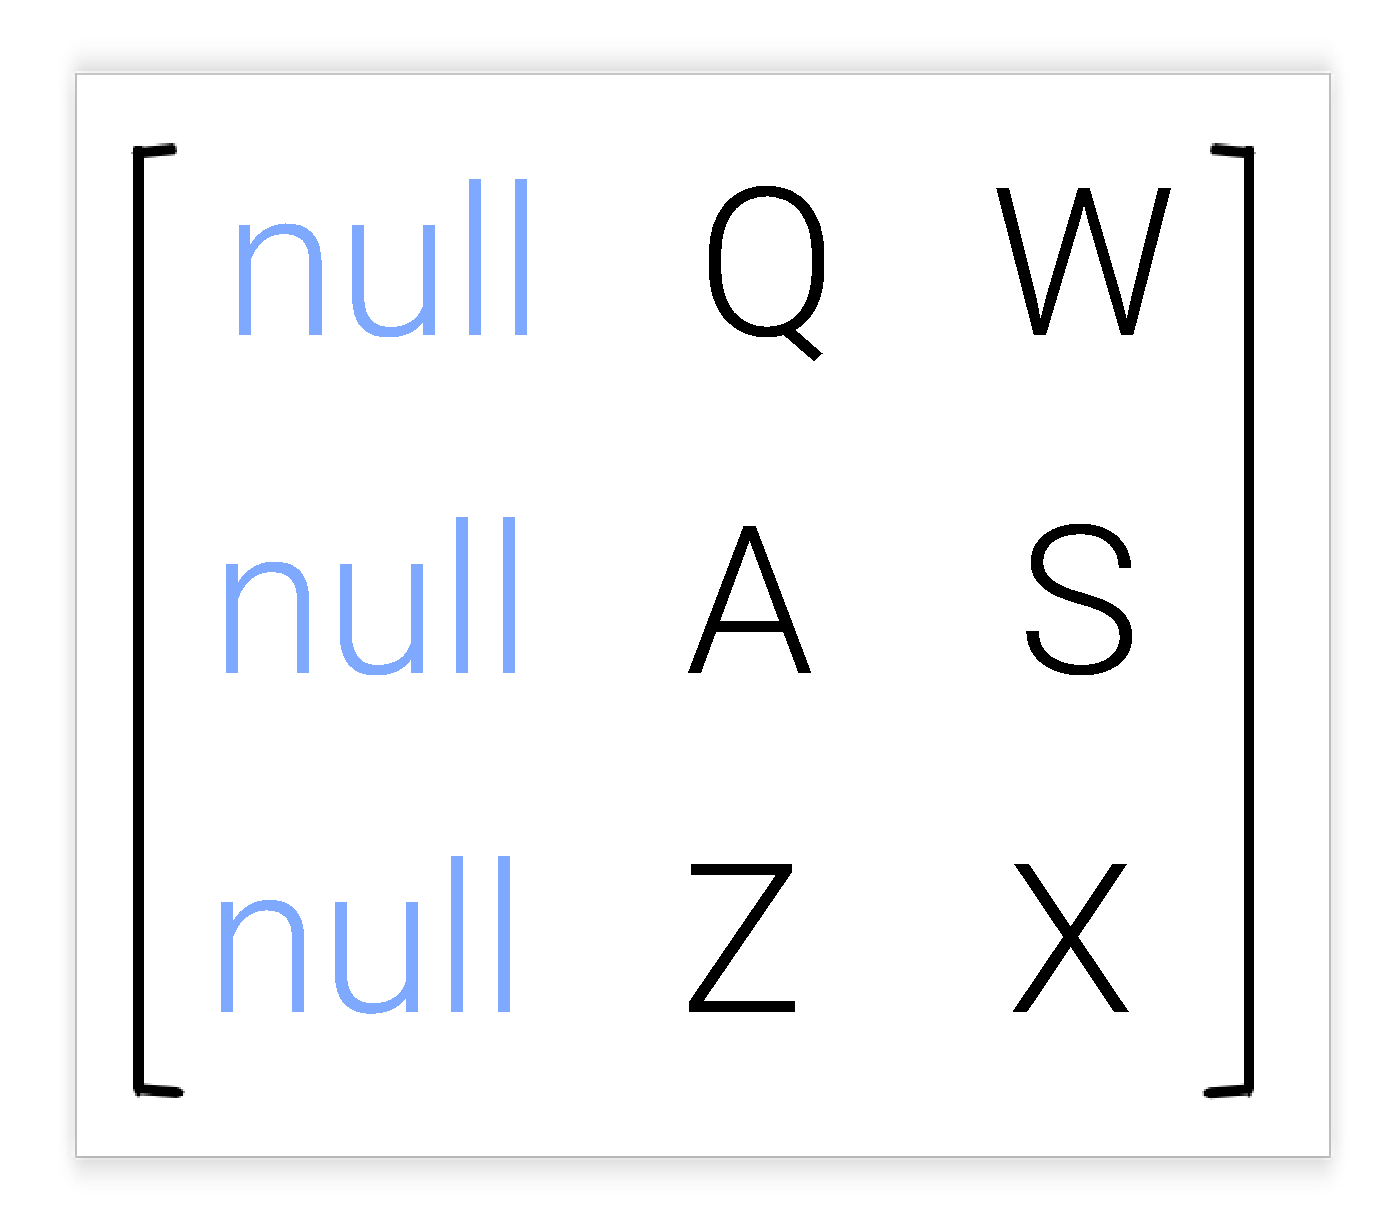
\includegraphics[width=.3\textwidth]{neighbor_matrix.pdf}} \hspace{35pt}
\subfloat[][Gaussian distribution \label{gaussianD}]
{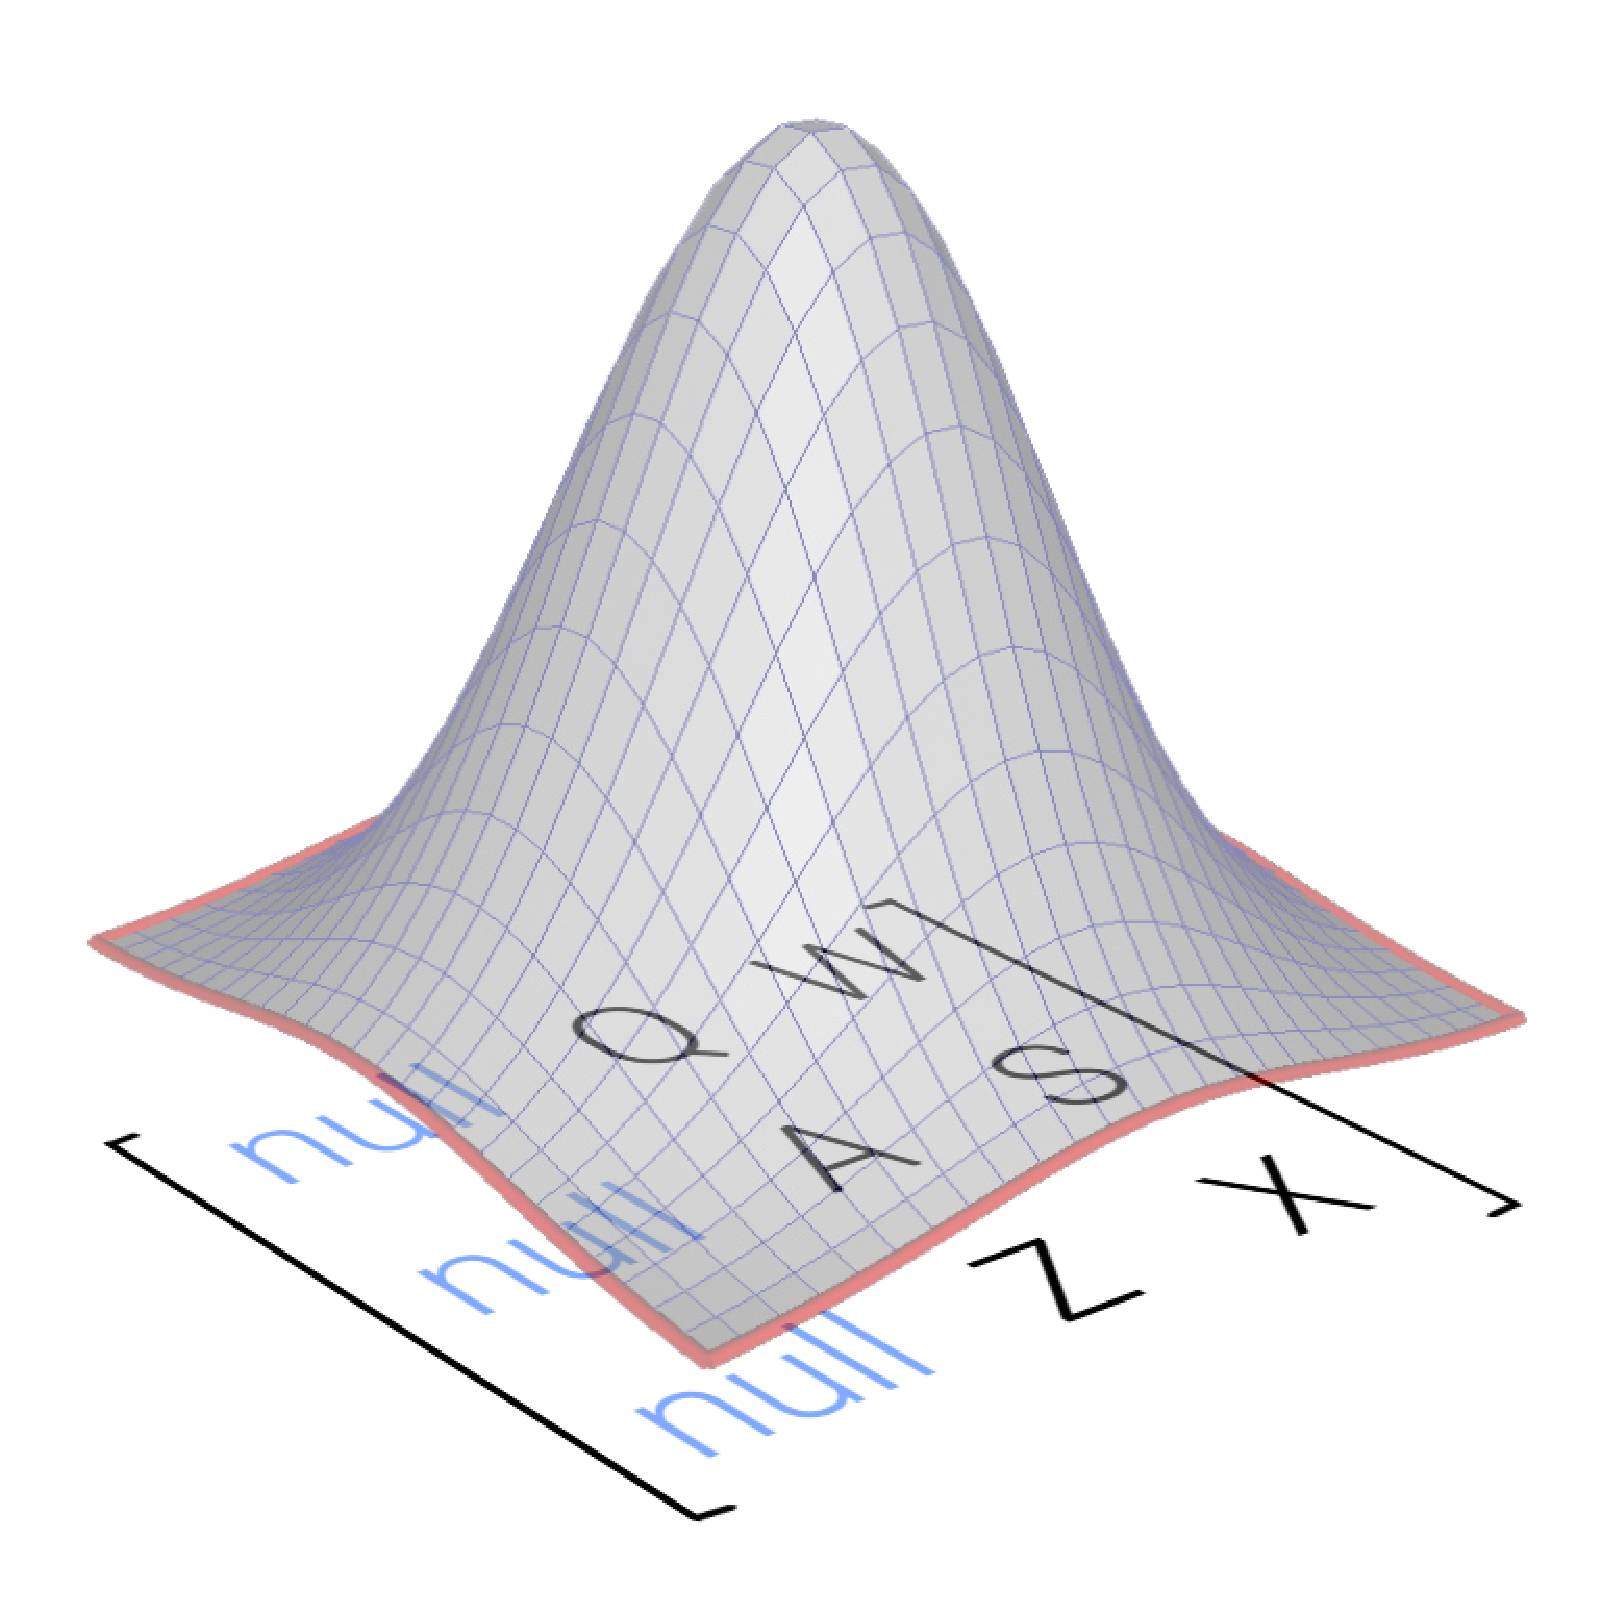
\includegraphics[width=.3\textwidth]{3D_Gaussian_Perspective.pdf}} \\
\caption{Emission distribution example}
\label{matrices}
\end{figure}


\newpage
\section{Tools and libraries}\label{libraries}
% Table generated by Excel2LaTeX from sheet 'Foglio3'
\begin{table}[htbp]
  \centering
  \caption{Libraries}
  \setlength{\tabcolsep}{0.4em}
    \begin{tabularx}{\linewidth}{XlX}
    \toprule
    Library & Source & Description \\
    \midrule
    Hidden-Markov Model &  \url{github.com/Red-devilz/hidden_markov}
    & Python implementation of the hidden markov model \\
    \midrule
    Autowrong & \url{github.com/pwrstudio/autowrong} & introduces keyboard
    typos into a string \\
    \midrule
    Tweepy & \url{www.tweepy.org} & Python library for accessing the Twitter
    API.
    \\
    \bottomrule
    \end{tabularx}%
  \label{tab:libraries}%
\end{table}%

% \begin{tabular}{ll}
% Mass of empty crucible & \SI{7.28}{\gram}\\
% Mass of crucible and magnesium before heating & \SI{8.59}{\gram}\\
% Mass of crucible and magnesium oxide after heating & \SI{9.46}{\gram}\\
% Balance used & \#4\\
% Magnesium from sample bottle & \#1
% \end{tabular}

%----------------------------------------------------------------------------------------
%	SECTION 3
%----------------------------------------------------------------------------------------



% \begin{tabular}{ll}
% Mass of magnesium metal & = \SI{8.59}{\gram} - \SI{7.28}{\gram}\\
% & = \SI{1.31}{\gram}\\
% Mass of magnesium oxide & = \SI{9.46}{\gram} - \SI{7.28}{\gram}\\
% & = \SI{2.18}{\gram}\\
% Mass of oxygen & = \SI{2.18}{\gram} - \SI{1.31}{\gram}\\
% & = \SI{0.87}{\gram}
% \end{tabular}
% 
% Because of this reaction, the required ratio is the atomic weight of magnesium: \SI{16.00}{\gram} of oxygen as experimental mass of Mg: experimental mass of oxygen or $\frac{x}{1.31}=\frac{16}{0.87}$ from which, $M_{\ce{Mg}} = 16.00 \times \frac{1.31}{0.87} = 24.1 = \SI{24}{\gram\per\mole}$ (to two significant figures).

%----------------------------------------------------------------------------------------
%	SECTION 4
%----------------------------------------------------------------------------------------

\section{Data Analysis}\label{analysis}
\subsection{Dataset}\label{dataset}
Table~\ref{tab:dataset} reports the datasets used to realize our project: the
data were used both to train the model parameters and to test our algorithm. In
this report we refer to them as \emph{Twitter}~(collection of tweets about apple
and trump), \emph{Swift}~(collection of news, tweets and
blogs text) and \emph{Hybrid}~(Tweet + Swift).

All datasets were previously cleaned from all characters
different from the alphabetical ones(lowercase and uppercase), plus whitespace.
Moreover, urls and mentions were removed from each tweet in order to avoid
noisy samples.

\begin{table}[htbp]
  \centering
  \caption{Dataset information}
  \setlength{\tabcolsep}{0.4em}
  \renewcommand{\arraystretch}{1.2}
    \begin{tabular}{lcr}
    \toprule
    \textbf{Name}  & \textbf{Source} & \textbf{\#characters} \\
    \midrule
    news  & Swift Key  & 204233394 \\
    twitter & Swift Key  & 164456394 \\
    blogs & Swift Key  & 207723793 \\
    apple & Twitter & 2376252 \\
    trump & Twitter & 11849767 \\
    \bottomrule
    $Swift$ & news, twitter, blogs & 576413581 \\
    $Twitter$ & apple, trump & 14226019 \\
    $Hybrid$ & Swift, Twitter & 590639600 \\
    \bottomrule
    \end{tabular}%
  \label{tab:dataset}%
\end{table}%



We partitioned the output data by assigning each data three boolean
attributes:

\textit{1)} \emph{Perturbed}, which indicates whether the data was
perturbed by Autowrong or not; \textit{2)}
\emph{Corrected}, set to $1$ if the model tried to correct it; \textit{3)}
\emph{True}, set to $1$ if the output data matches the ground truth.
In Figure~\ref{confusionCircle} we reported the representation of how we divided the data.
the circle contains all data which were corrected(\emph{Corrected} = $1$) by our
model.
It is divided in:
\begin{itemize} 
	\item \textbf{corrected-right}: perturbed data which were corrected and match
	the ground truth;
	\item \textbf{corrected-wrong}: data which were corrected badly whether they
	were perturbed or not;
	\item \textbf{not corrected-right}: data not corrected and match the
	ground truth;
	\item \textbf{not corrected-wrong}: missed correction of data.
\end{itemize}

In Table~\ref{tab:features}, all the possible combination of attributes which
define each data set.



\begin{figure}[hbp]
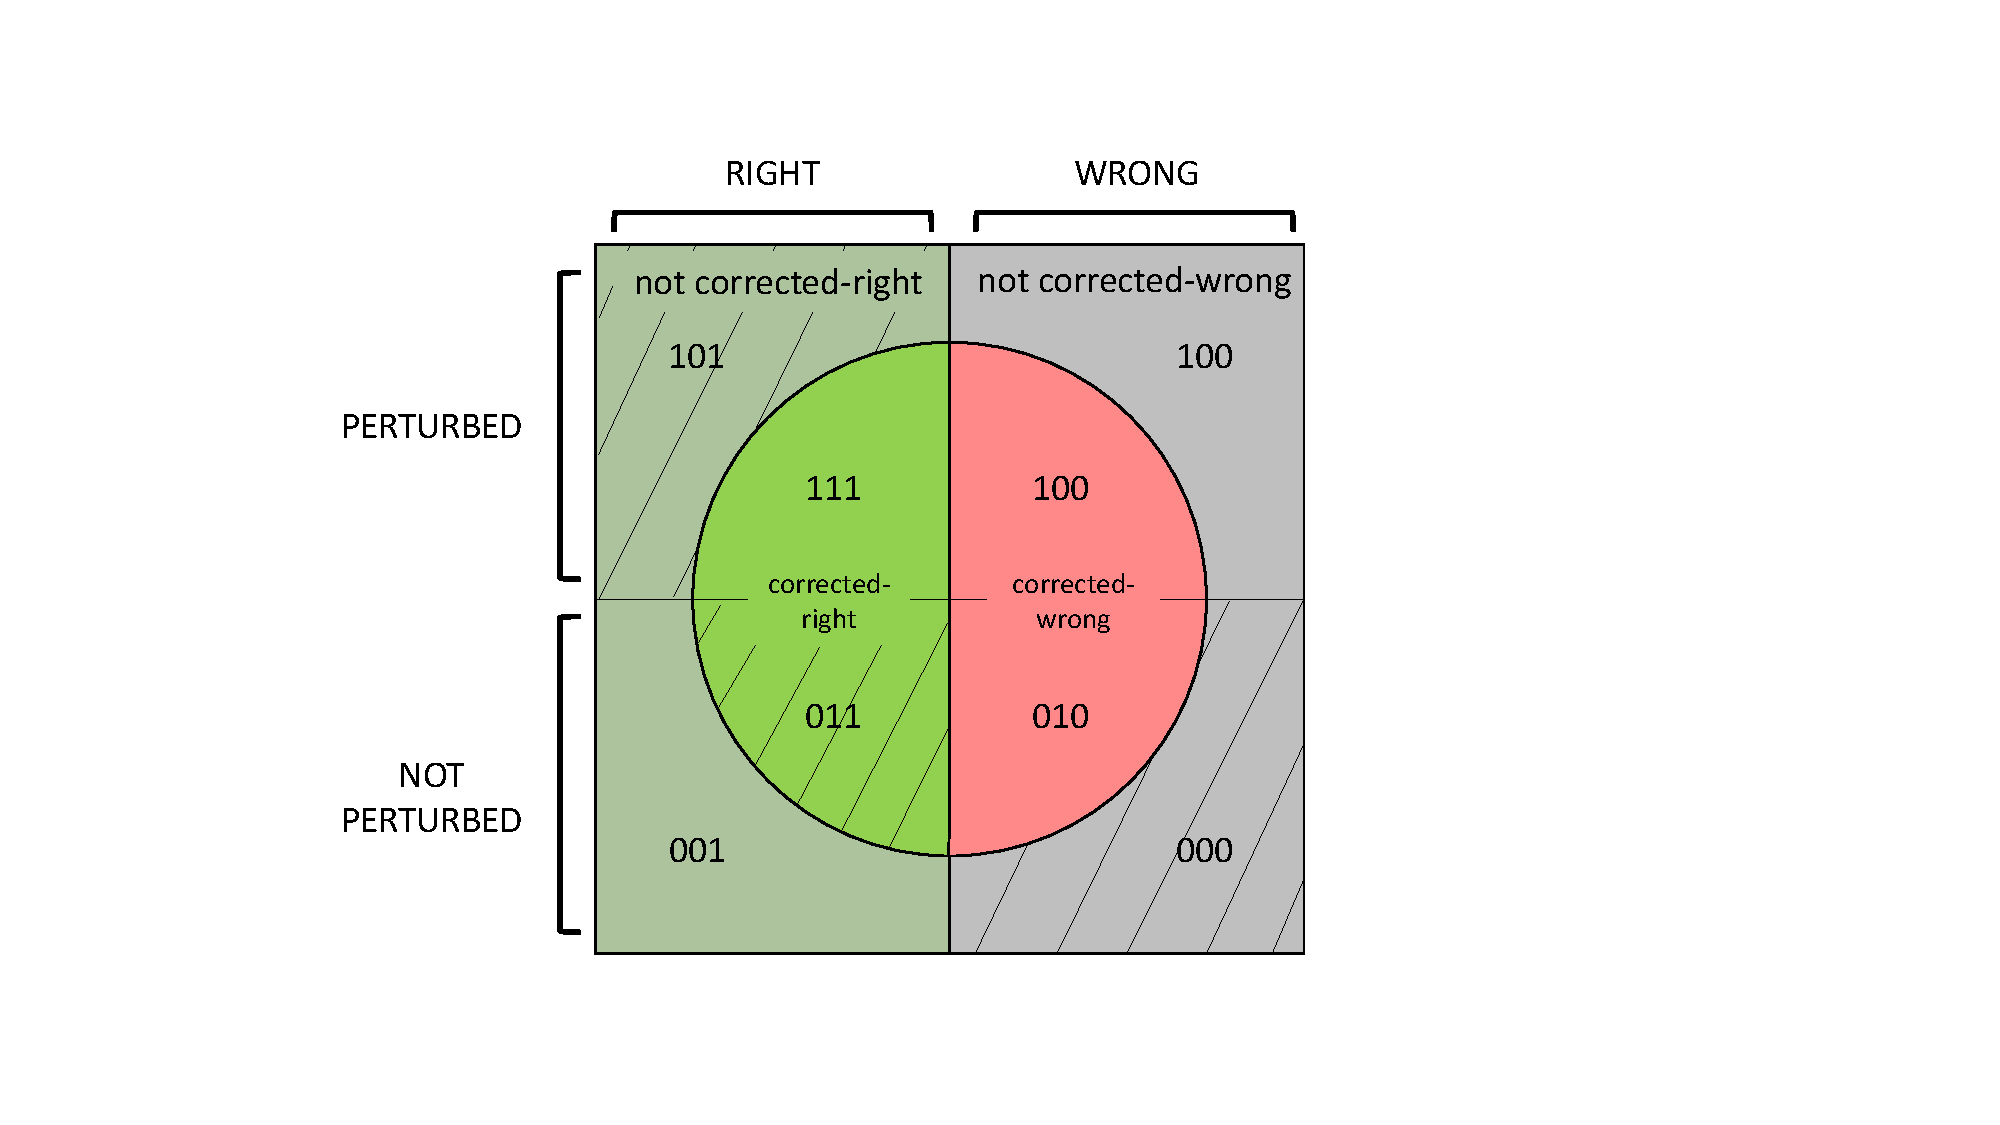
\includegraphics[width=\linewidth,clip=true,trim=100 30 150
60]{confusionCircle.pdf}
\caption{Data representation}
\label{confusionCircle}
\end{figure}


% Table generated by Excel2LaTeX from sheet 'Foglio2'
\begin{table}[htbp]
  \centering
  \caption{Data attributes}
    \begin{tabularx}{\linewidth}{ccc|cc}
    %\toprule
    \multicolumn{3}{c}{\textbf{Observation}} &       &  \\
    \midrule
    \textbf{Perturbed} & \textbf{Corrected} & \textbf{True} & \textbf{Description} & \textbf{Evaluation} \\
    \midrule
    0     & 0     & 0     &   -    & impossible \\
    0     & 0     & 1     & not altered observation & correct \\
    0     & 1     & 0     & unnecessary correction & wrong \\
    1     & 0     & 0     & missed correction & wrong \\
    1     & 0     & 1     &   -    & impossible \\
    1     & 1     & 0     & wrong correction & wrong \\
    0     & 1     & 1     &   -    & impossible \\
    1     & 1     & 1     & right  correction & correct \\
    \bottomrule
    \end{tabularx}%
  \label{tab:features}%
\end{table}%

% Table generated by Excel2LaTeX from sheet 'Foglio5'
% Table generated by Excel2LaTeX from sheet 'Foglio5'
% Table generated by Excel2LaTeX from sheet 'Foglio5'
\begin{table}[htbp]
  \centering
  \caption{Confusion matrix}
  \setlength{\tabcolsep}{1em}
  \renewcommand{\arraystretch}{1.5}
    \begin{tabular}{cccc}
    \toprule
          &       & \multicolumn{2}{c}{\textbf{Predicted condition}} \\
    \midrule
          &       & T     & F \\
    \multicolumn{1}{c}{\multirow{2}[0]{*}{\textbf{True Condition}}} & T     &
    111 & 100 \\
    \multicolumn{1}{c}{} & F     & {010, 110} & 001 \\
    \bottomrule
    \end{tabular}%
  \label{tab:confusionM}%
\end{table}%

%


%frequency table
%graphs
\section{Test}

\section{Demo and GUI}
%insert screenshot
As result of our project, we introduce our demo ``HMMispelling''. The demo
offers a Graphic User Interface and two modes: an interactive mode where the
user can type his message and check the real time correction and an automatic
one which shows the real time correction of a stream of real tweets.

\section{Conclusions}

% The atomic weight of magnesium is concluded to be \SI{24}{\gram\per\mol}, as determined by the stoichiometry of its chemical combination with oxygen. This result is in agreement with the accepted value.
% 
% \begin{figure}[h]
% \begin{center}
% %%\includegraphics[width=0.65\textwidth]{placeholder} % Include the image
% % placeholder.png
% \caption{Figure caption.}
% \end{center}
% \end{figure}
% 
% %----------------------------------------------------------------------------------------
% %	SECTION 5
% %----------------------------------------------------------------------------------------
% 
% \section{Discussion of Experimental Uncertainty}
% 
% The accepted value (periodic table) is \SI{24.3}{\gram\per\mole} \cite{Smith:2012qr}. The percentage discrepancy between the accepted value and the result obtained here is 1.3\%. Because only a single measurement was made, it is not possible to calculate an estimated standard deviation.
% 
% The most obvious source of experimental uncertainty is the limited precision of the balance. Other potential sources of experimental uncertainty are: the reaction might not be complete; if not enough time was allowed for total oxidation, less than complete oxidation of the magnesium might have, in part, reacted with nitrogen in the air (incorrect reaction); the magnesium oxide might have absorbed water from the air, and thus weigh ``too much." Because the result obtained is close to the accepted value it is possible that some of these experimental uncertainties have fortuitously cancelled one another.
% 
% %----------------------------------------------------------------------------------------
% %	SECTION 6
% %----------------------------------------------------------------------------------------
% 
% \section{Answers to Definitions}
% 
% \begin{enumerate}
% \begin{item}
% The \emph{atomic weight of an element} is the relative weight of one of its atoms compared to C-12 with a weight of 12.0000000$\ldots$, hydrogen with a weight of 1.008, to oxygen with a weight of 16.00. Atomic weight is also the average weight of all the atoms of that element as they occur in nature.
% \end{item}
% \begin{item}
% The \emph{units of atomic weight} are two-fold, with an identical numerical value. They are g/mole of atoms (or just g/mol) or amu/atom.
% \end{item}
% \begin{item}
% \emph{Percentage discrepancy} between an accepted (literature) value and an experimental value is
% \begin{equation*}
% \frac{\mathrm{experimental\;result} - \mathrm{accepted\;result}}{\mathrm{accepted\;result}}
% \end{equation*}
% \end{item}
% \end{enumerate}

%----------------------------------------------------------------------------------------
%	BIBLIOGRAPHY
%----------------------------------------------------------------------------------------

\bibliographystyle{apalike}

\bibliography{sample}

%----------------------------------------------------------------------------------------


\end{document}
